\documentclass[IN,english]{tumbook}
\usepackage{tabularx}
%\usepackage[utf8]{inputenc}
%\usepackage[T1]{fontenc}
%\usepackage{graphicx}
%\usepackage{amsmath}

\makeindex

% Information for the title page
\Seminar{Software Engineering for Business Applications - Master}
\Semester{SS 2015}
\title{Business Model for the Web Application \emph{Travel Diary}}
\Untertitel{}
\Themensteller{Prof. Dr. Florian Matthes}
\Autorenadresse{}
\Matrikelnummer{}
\Fachsemester{}
\Abgabetermin{3. July 2015}
\author{Mantosh Kumar, Ulrike Niemann, Albert Steckermeier}
\date{3. July 2015}



\begin{document}

\maketitle
\newpage
\tableofcontents
\newpage

\chapter{Use Case 1: Searching for Vacations}

Users can search for vacations in \emph{Travel Diary} using keywords. The website uses a search input in the navigation part at the top of the page. Only keywords can be selected. Keywords can by added by starting to type into the search bar and selecting one of the keywords provided by the auto-completion of the search input. Furthermore the user is provided with some inspiration for possible keywords below the search bar. The keywords below the search bar can be added by clicking on the keyword chips. They will then be added to the current selection of keywords in the search bar at the top of the page. Keywords can be removed by clicking the keyword chip in the search bar. Figure \ref{fig:search-keywords} shows a possible search state. Furthermore below the search bar there is a tab which can be used to specify a budget limit. It includes a slider as well as an input field for the budget. Figure \ref{fig:search-budget} shows the budget tab for the search.

\begin{figure}
	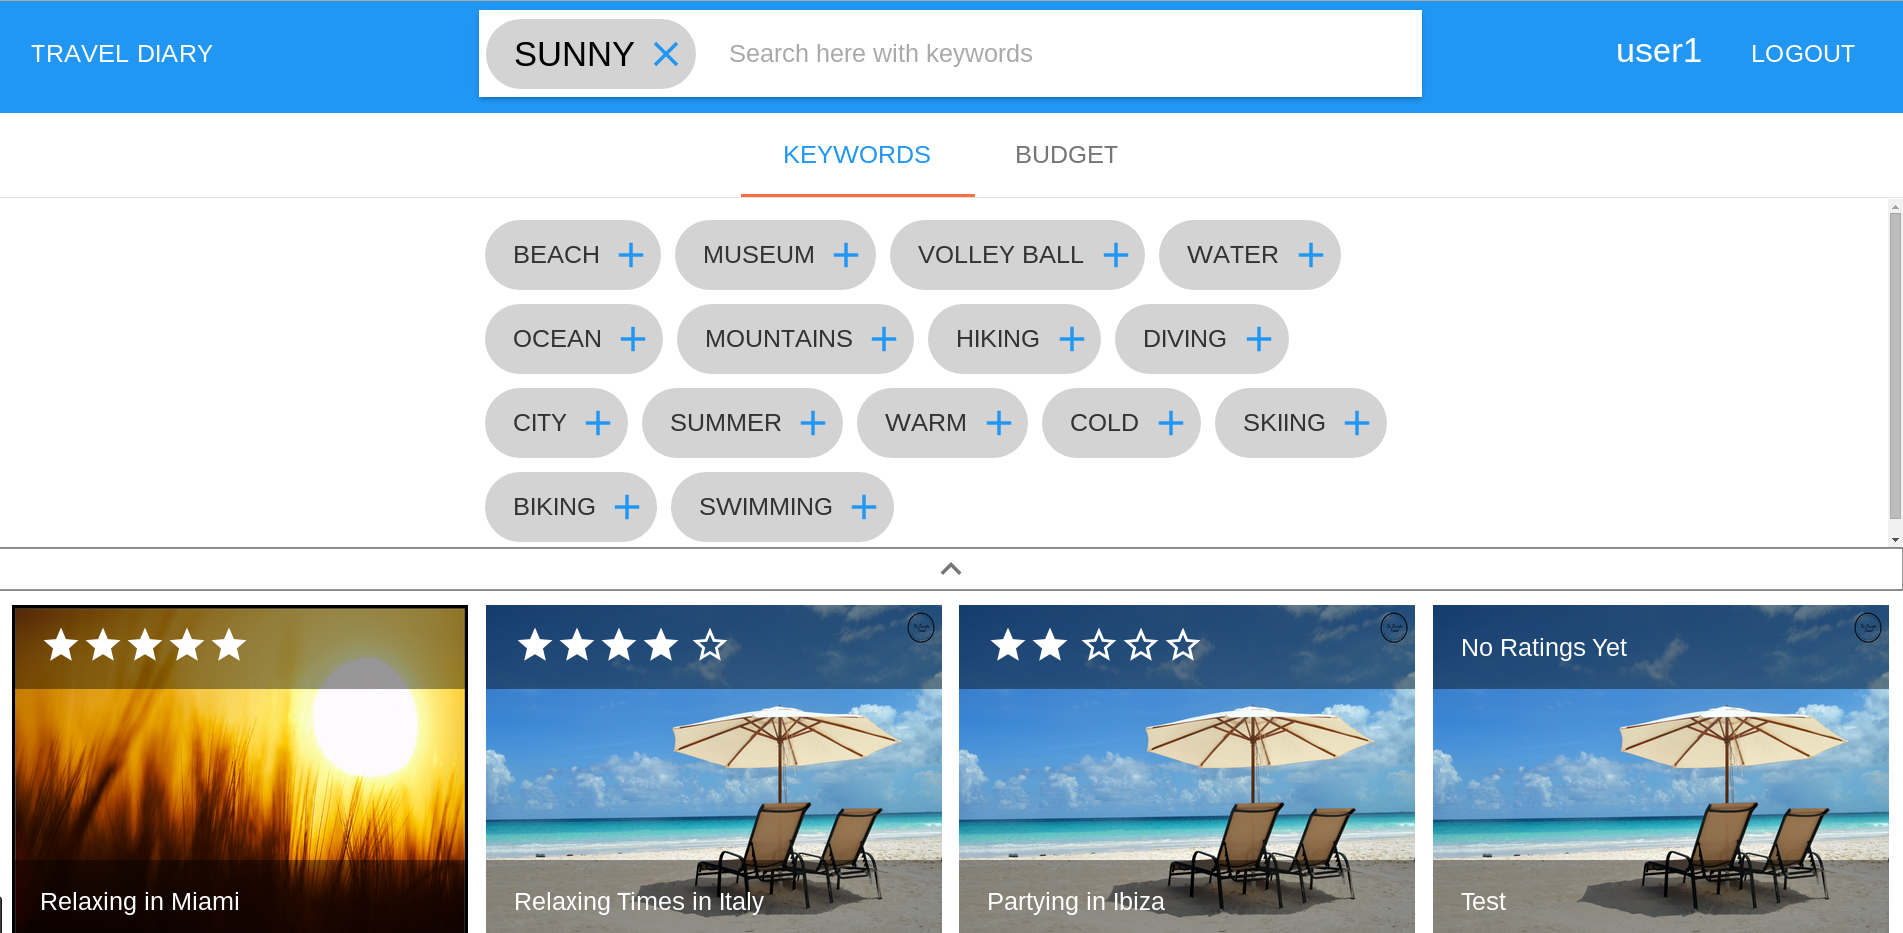
\includegraphics[width=\textwidth]{pictures/vacation-search-keywords}
	\caption{Search of vacations with keywords.}
	\label{fig:search-keywords}
\end{figure}

\begin{figure}
	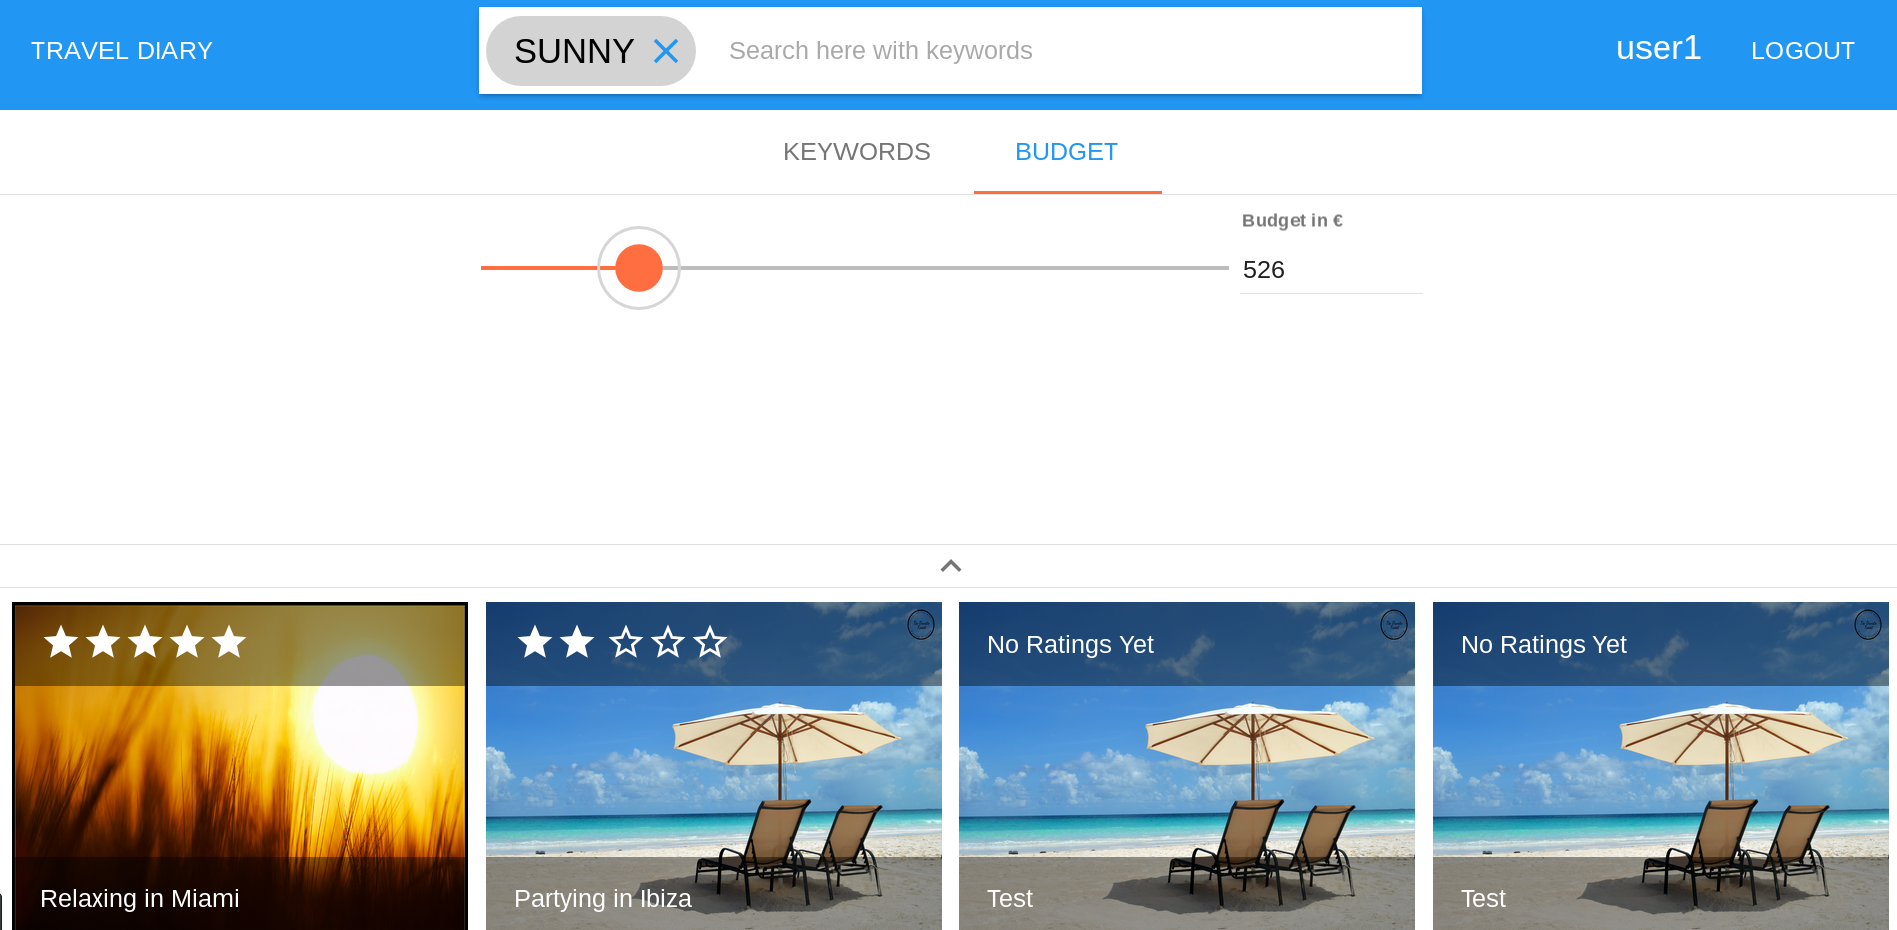
\includegraphics[width=\textwidth]{pictures/vacation-search-budget}	
	\caption{Budget option for vacation search.}
	\label{fig:search-budget}
\end{figure}

\chapter{Use Case 2: Sharing the Experience of an Activity}

Users share their experience by writing a review for the activity. For that purpose the activity details view has a \emph{My Review} button in the top right corner. There the user can manage his review for that activity. A dropdown menu offers the option to add a review or edit/delete it if the user has already written one. Adding or editing a review shows a dialog with a form for the title, description and rating of the review. The form validates that the title and description is not empty. Furthermore it requires the user to provide a rating. Figure \ref{fig:dialog-activity-review} shows the dialog with the activity details view in the background.

\begin{figure}
	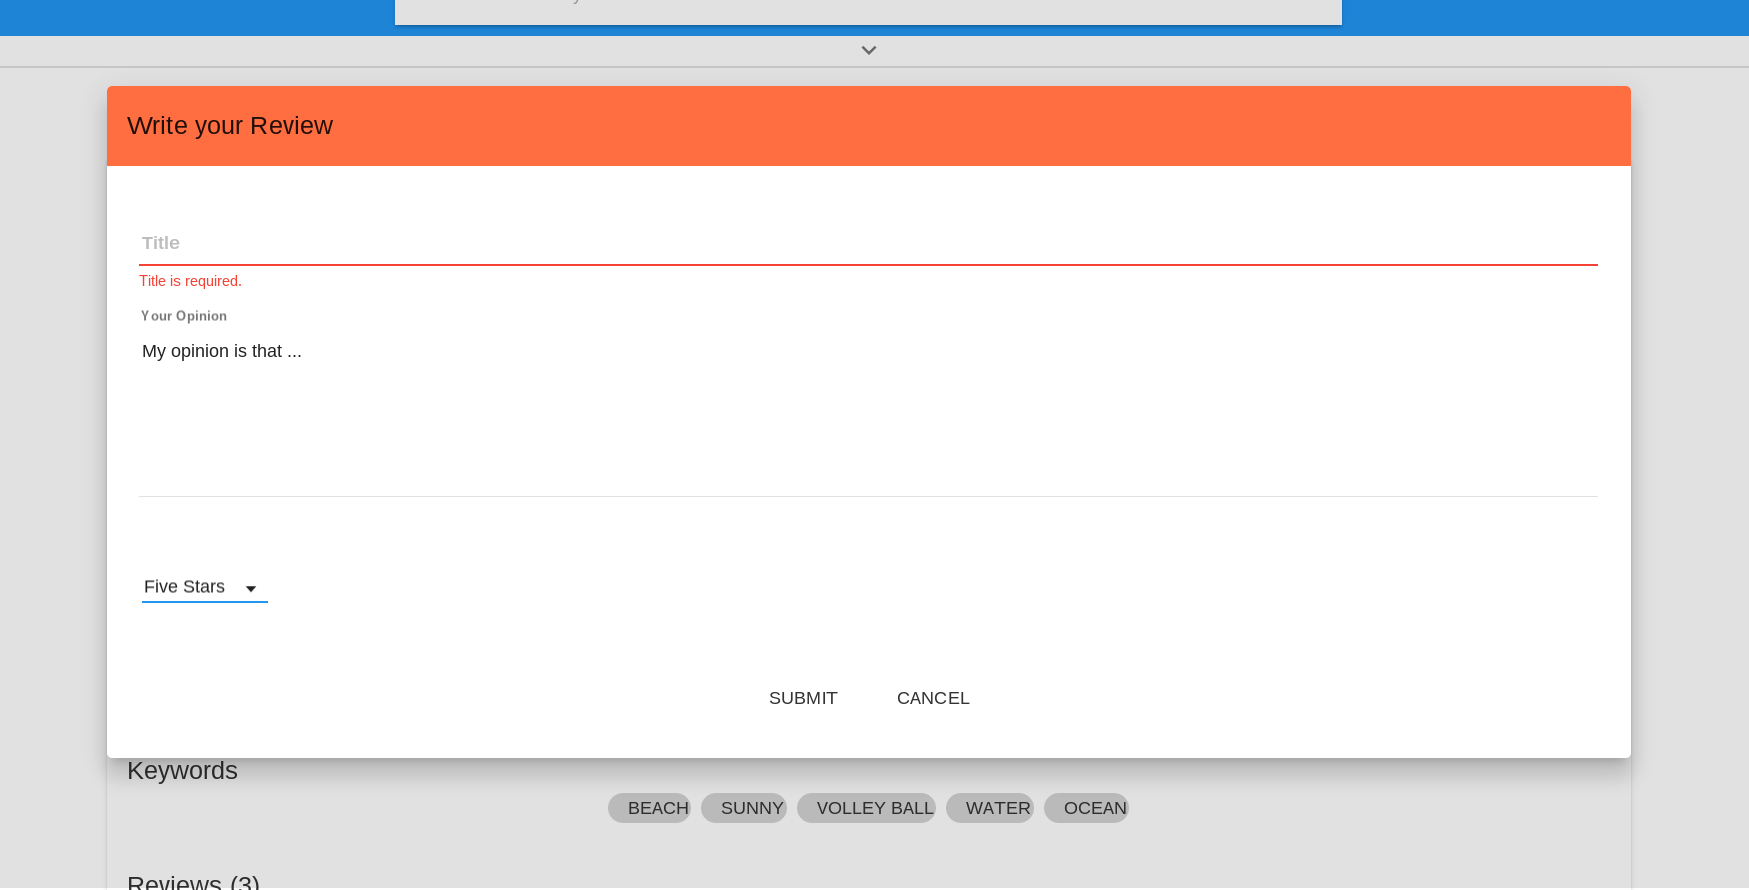
\includegraphics[width=\textwidth]{pictures/review-activity}
	\caption{Dialog for adding a review to an activity.}
	\label{fig:dialog-activity-review}
\end{figure}

\chapter{Use Case 3: Sharing the Experience of a Vacation}

Sharing the experience of a vacation works analogously to use case 2. The user provides a review as well. The vacation details page also has an \emph{My Review} button to add, edit or delete the users review. Figure \ref{fig:dialog-vacation-review} shows the dialog with the vacation details view in the background.

\begin{figure}
	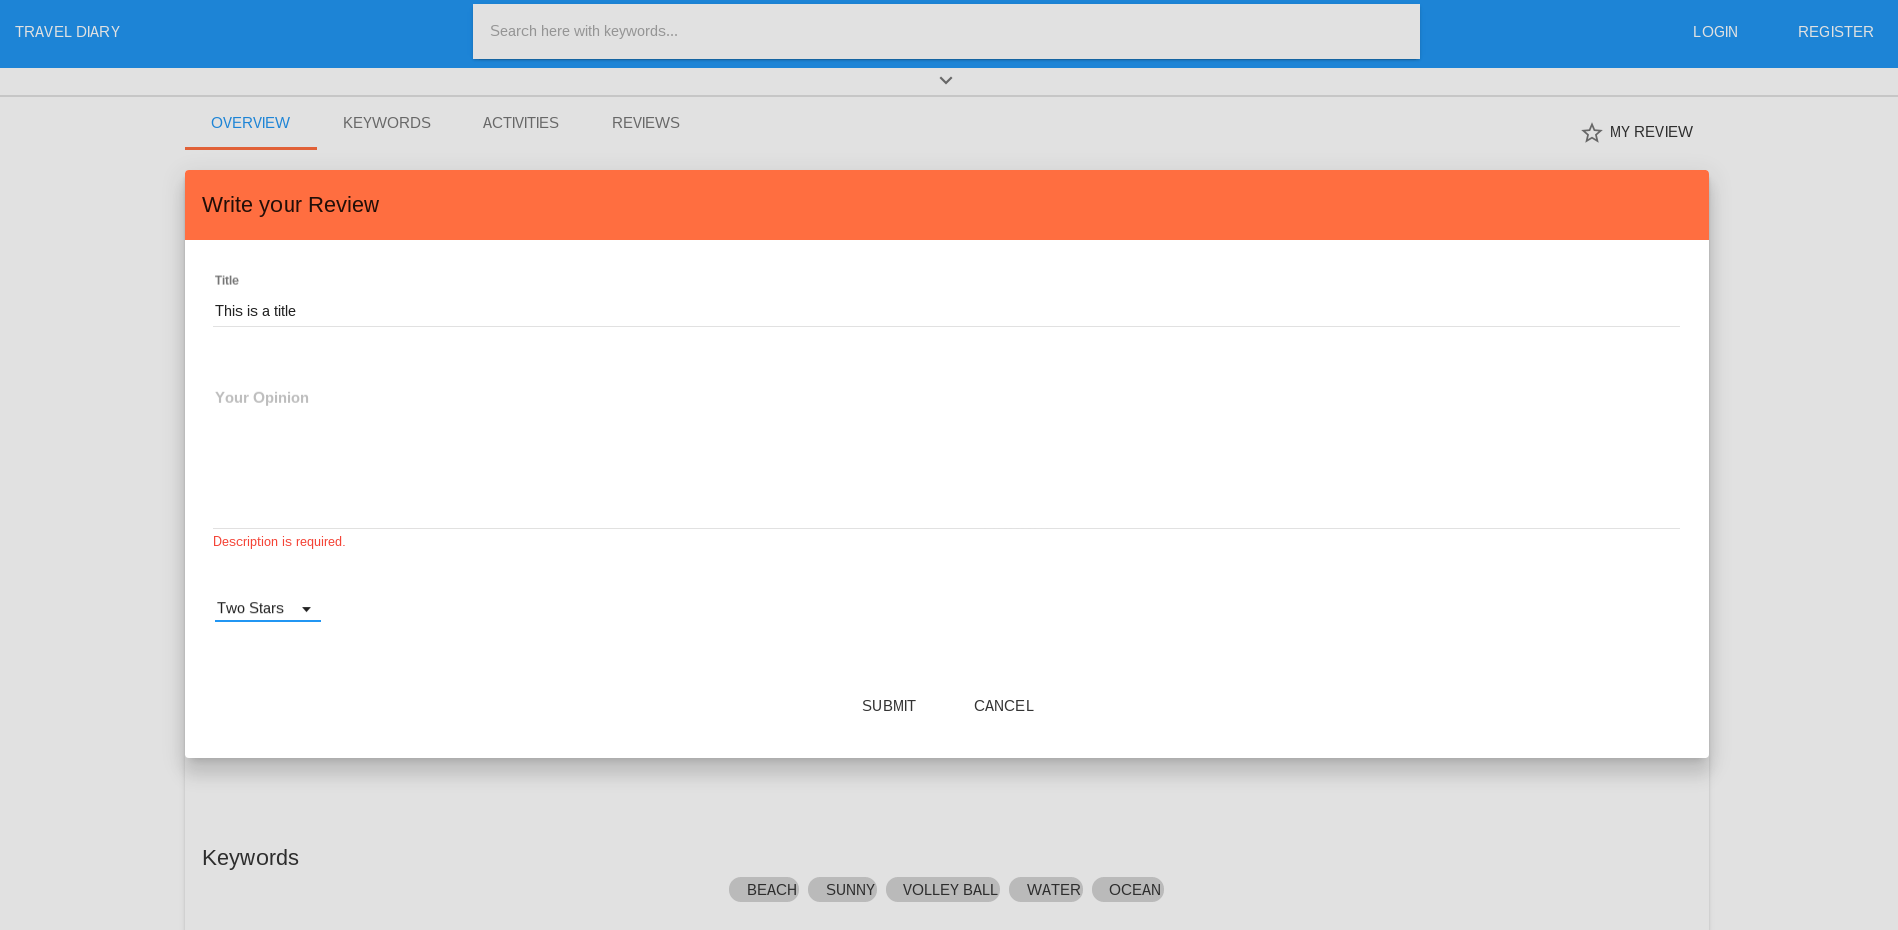
\includegraphics[width=\textwidth]{pictures/review-vacation}
	\caption{Dialog for adding a review to a vacation.}
	\label{fig:dialog-vacation-review}
\end{figure}

\chapter{Use Case 4: Planning a Vacation}
Planning a Vacation should support the user in creating his dream vacation. First of all, the user has the opportunity to search for vacations that match his preferences by selecting fitting keywords and getting inspiration from other users. When the user finds a promising vacation, he can simply copy the vacation and modify it as he likes. For instance, he can search for and plan the Activities he wants to attend during the vacation. Furthermore, the user can plan his Budget for the journey and book flights or an accommodation via affiliates.
During the vacation or after the user returns home, he can add pictures and descriptions of his experiences and impressions and share this with the travel diary community. Figures \ref{fig:vacation-details-1} and \ref{fig:vacation-details-2} show the vacation details view. The edit view of a vacation is depicted in figures \ref{fig:vacation-edit-1} and \ref{fig:vacation-edit-2}.


\begin{figure}
	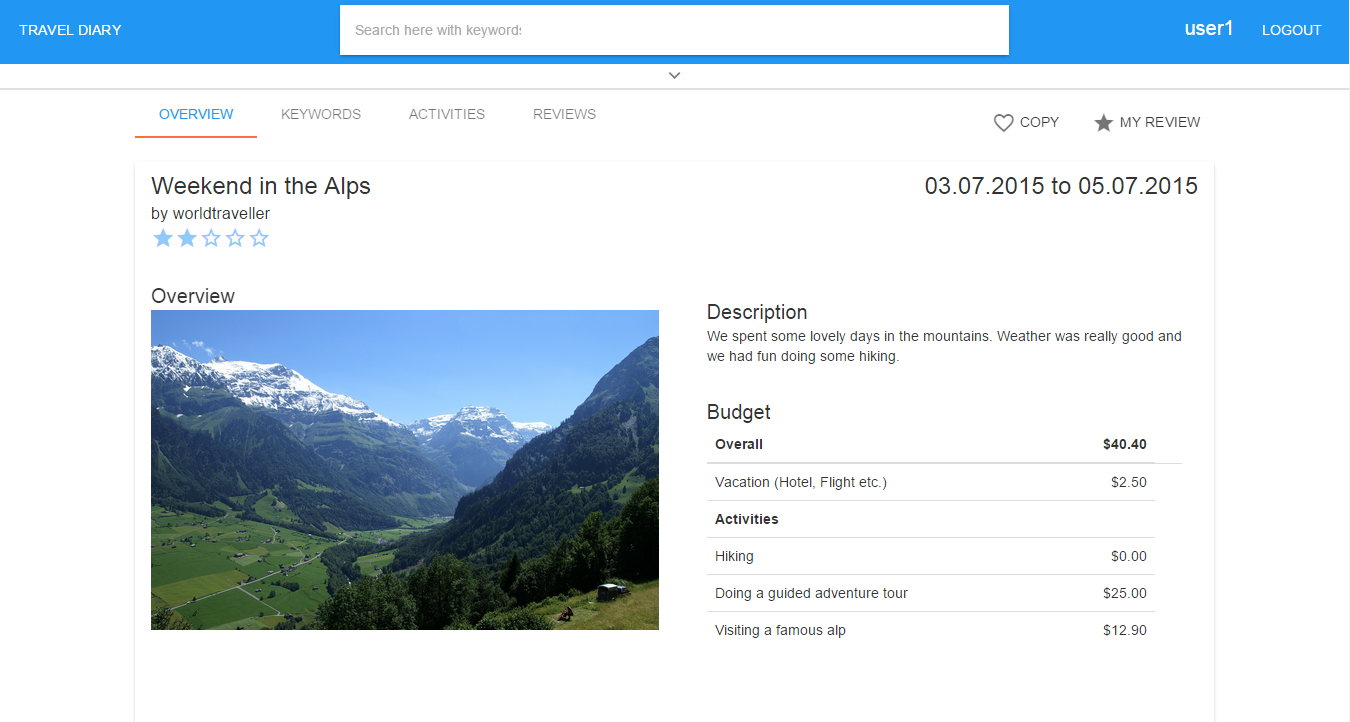
\includegraphics[width=\textwidth]{pictures/UseCase4_1}
	\caption{Details view of a vacation.}
	\label{fig:vacation-details-1}
\end{figure}

\begin{figure}
	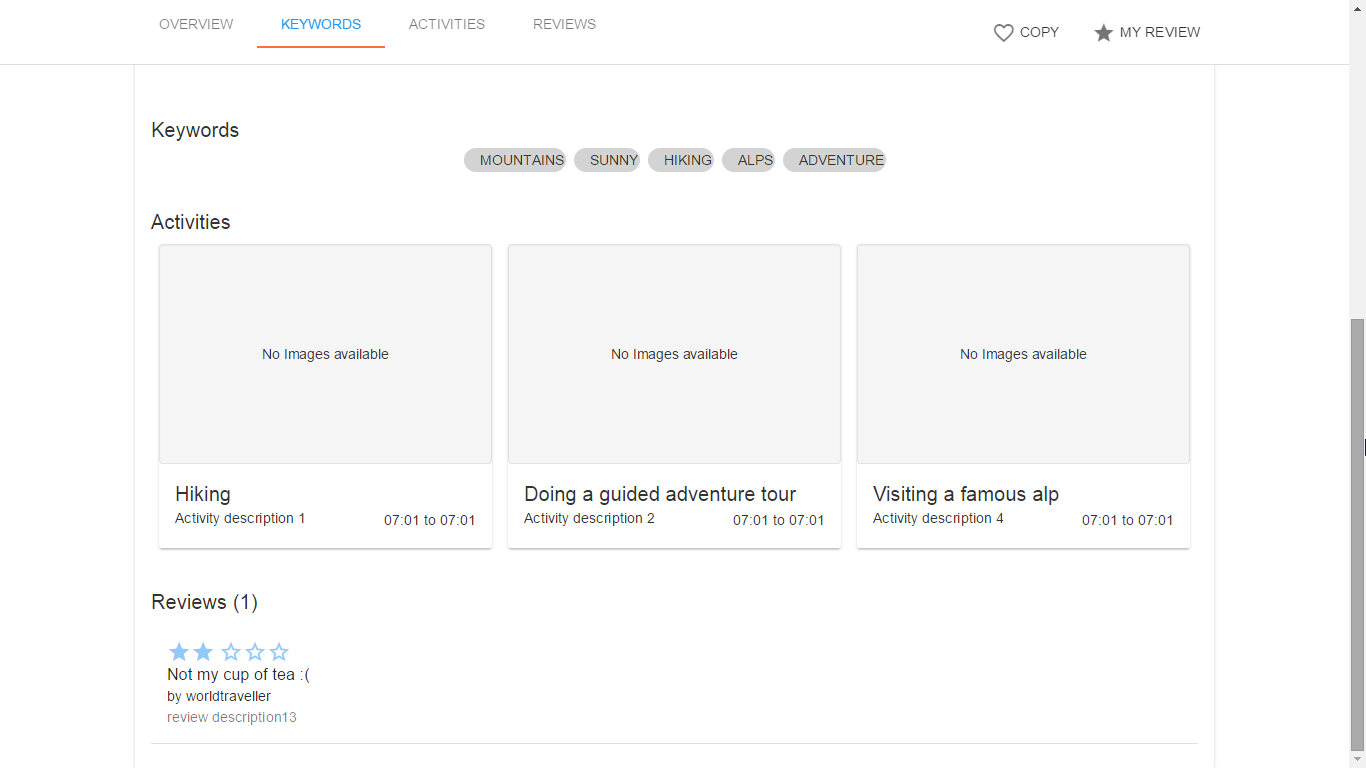
\includegraphics[width=\textwidth]{pictures/UseCase4_2}	
	\caption{Activities and Reviews part of the vacation details view.}
	\label{fig:vacation-details-2}
\end{figure}

\begin{figure}
	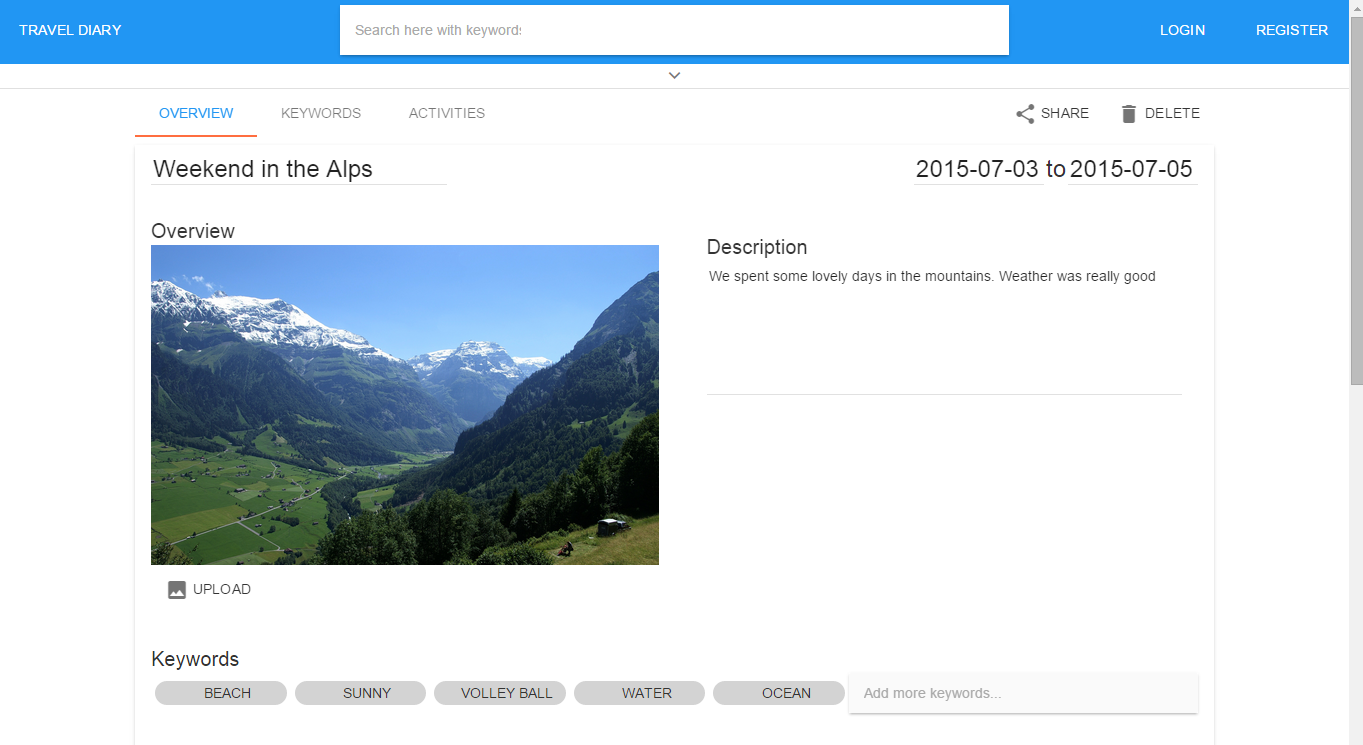
\includegraphics[width=\textwidth]{pictures/UseCase4_3}
	\caption{Top part of the edit view for vacations.}
	\label{fig:vacation-edit-1}
\end{figure}

\begin{figure}
	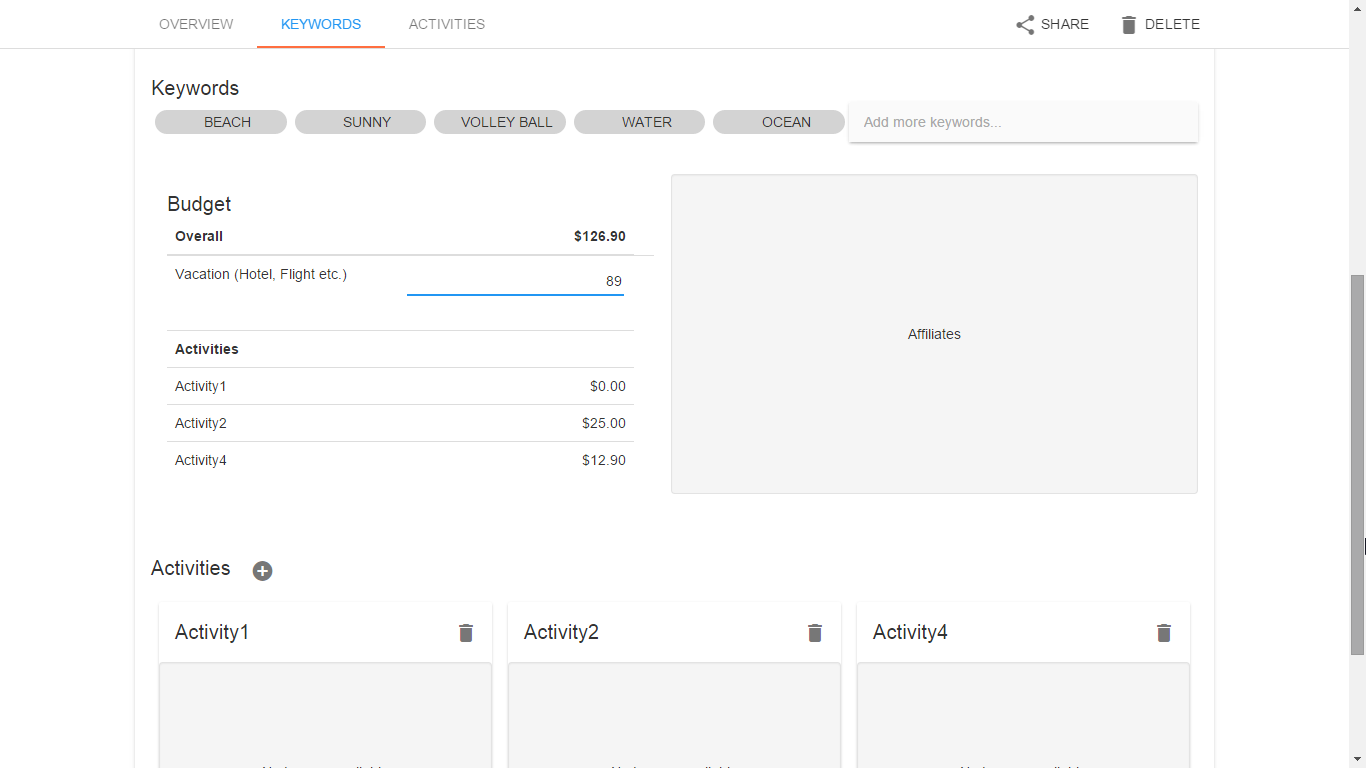
\includegraphics[width=\textwidth]{pictures/UseCase4_4}
	\caption{Bottom part of the edit view for vacations.}
	\label{fig:vacation-edit-2}
\end{figure}

\end{document}
